\documentclass[11pt]{article}

\usepackage[letterpaper,bindingoffset=0.2in,
            left=1in,right=1in,top=1in,bottom=1in,
            footskip=.25in]{geometry}

\usepackage{hyperref}
	\hypersetup{
			colorlinks=true,
			linkcolor=black,
			filecolor=magenta,      
			urlcolor=blue,
	}
	
\usepackage{graphicx}
	\graphicspath{ {images/} }
	
\usepackage{subcaption}
	
\begin{document}


\title{COMP SCI 5401 FS2017 Assignment 2b}
\author{Stuart Miller\\\href{mailto:sm67c@mst.edu}{sm67c@mst.edu}}
\maketitle


\section{Overview}\label{sect:overview}

Assignment 2b provides an improvement to the Iterative Prisoner's Dilemma (IPD) problem by employing a Genetic Programming Search across single agents evaluated by a tit-for-tat strategy search. 


\section{Algorithm Strategy}\label{sect:alg_strat}
The algorithm works by generating a population of random trees (50\% full depth trees, 50\% grown tress), then iteratively generating children based on tree crossover from parents. Children are occasionally mutated, then simulated by playing tit-for-tat to obtain a fitness rating and added to the population. To obtain this fitness rating, each agents is plays a set number of rounds on a tit-for-tat strategy (the agent's opponent chooses what the agent itself did last). An option is also present to score each agent's fitness across multiple runs of IPD, with multiple randomized initial memories. Doing so allows for a more accurate fitness rating. After each generation, the population is thinned by removing poor agents chosen in a k-tournament. 

\section{Analysis}\label{sect:analysis}
The main problem with playing IPD tit-for-tat is that the agent very quickly learns that it can get into a pattern since the opponent is always guaranteed to do what it did last. It is very easy to an agent to get into a back-and-forth rhythm with its opponent with they simply alternate confessing and defecting. In such a way, all the agent has to do is choose what the opponent did an odd number of turns ago and it is guaranteed to score a 3 every time. Since there is a set number of startup round before payoffs are counted, the agent can establish this rhythm no matter what the initial memory is. This is evident in that the global best solution will almost always be O[1,3,5,...]. The agent is discouraged from branching out further because this would simply decrease its fitness do to the parsimony coefficient. The only way to break out of this would be to ditch the tit-for-tat strategy and implement a co-evolutionary approach. Perhaps even playing the against against a randomized opponent would fare better.

This fallacy is visible in Figure \ref{fig:default}. Notice how the best run simply approaches 3 (minus the minimal parsimony deduction for have a very small tree). Also notice how useless the boxplot is due to the non-diverse final population. There are only three possible fitness values. The all scored the same but had different parsimony penalties for size 1, 2, or 3 trees.

\begin{figure}[ht]
\centering
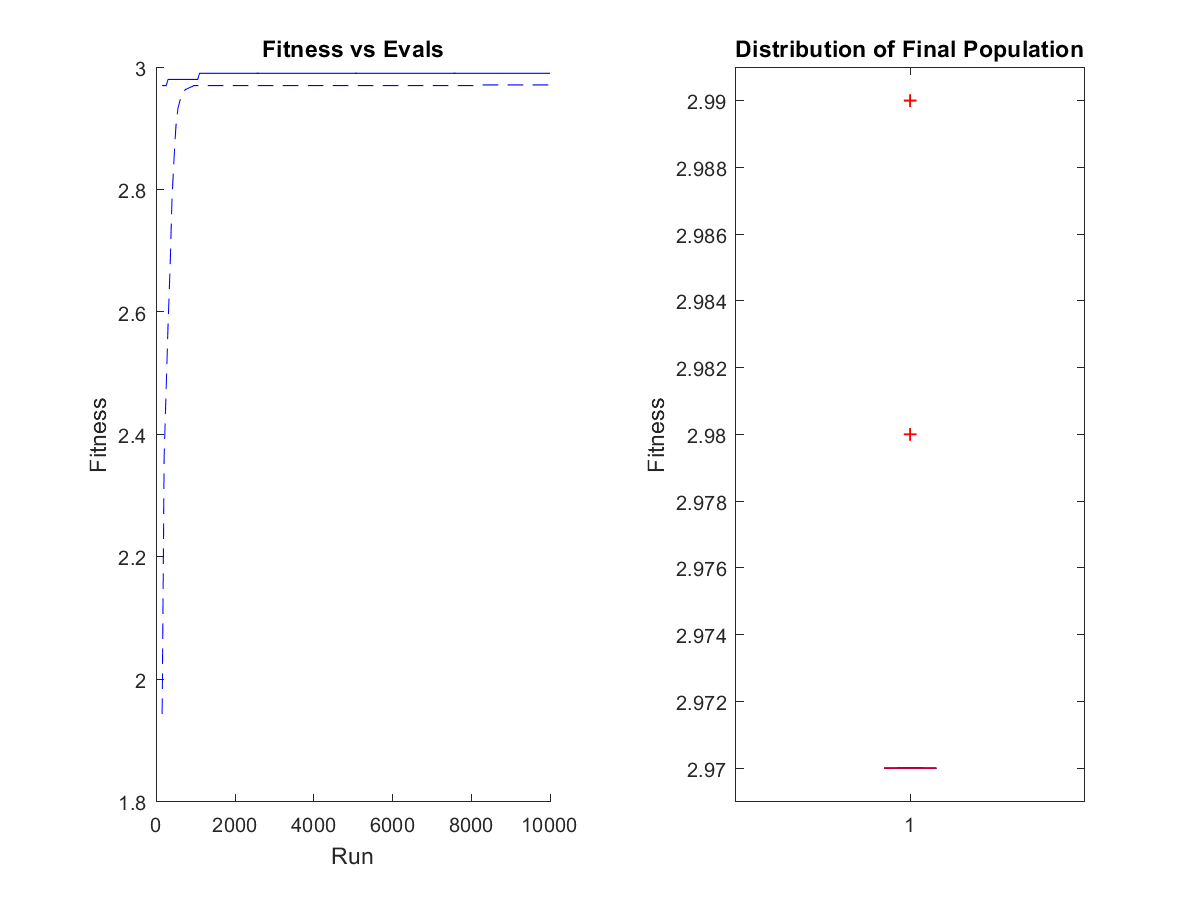
\includegraphics[width=6in]{default.png}
\captionof{figure}{Plot of Best Run }
\label{fig:default}
\end{figure}

\section{Analysis vs. Random Search}\label{sect:vs_random}

Figure \ref{fig:stats} shows the statistical analysis for the average final best fitness per run. Keep in mind that the Assn2b (Variable 2) results inclued the parsimony coefficient whereas the Assn2a (Variable 1) are raw average of the payoff. Assn2a saw higher averages as it was occasionally able to get up to a 5 payoff at the end, where Assn2b only ever settled on a 3.  Conversely, though Assn2b got to a 3 (minus parsimony) every single time while Assn2a often couldn't get past a best of 1. These averages prove that the approaches are roughly equal. Assn2b is more stable, but suffers from the restrictions discussed earlier in Section \ref{sect:analysis}.

\begin{figure}[ht]
\centering
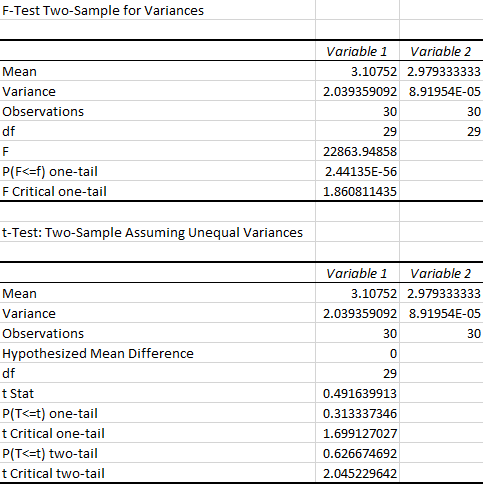
\includegraphics[width=3in]{stats.png}
\captionof{figure}{Statistical Analysis}
\label{fig:stats}
\end{figure}

\end{document}